\section{Linear System Identification}
\label{sec:sysid}

%% FIG: MODEL VS. WEIGHT OF L1 PENALTY (LASSO)
\begin{figure}
    \centering
    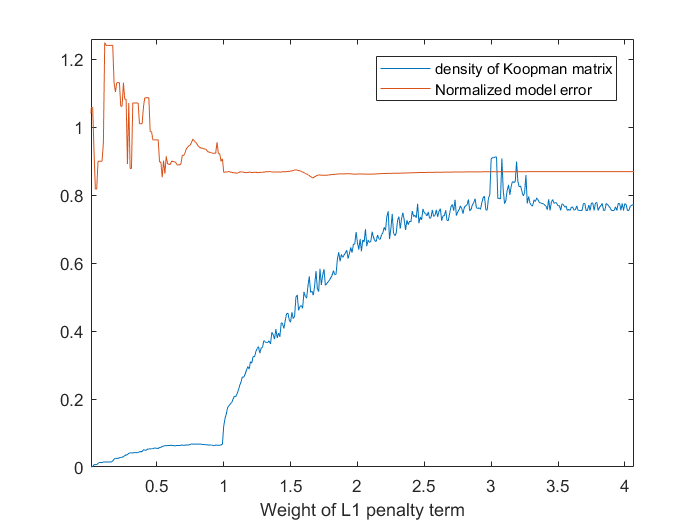
\includegraphics[width=\linewidth]{figures/lasso_placeholder.png}
    \caption{As the weight of the L1 penalty term increases, the Koopman operator matrix becomes more dense, and the model error decreases then levels off. This shows that there is a much sparser representation of the Koopman operator than the least-squares solution that generates a model of nearly identical accuracy.}
    \label{fig:lasso}
\end{figure}


%% Overview of this section
Any finite-dimensional nonlinear dynamical system has an equivalent infinite-dimensional linear representation in the space of real-valued functions of the system's state \cite{mauroy2016linear}.
In this function space, the (linear) Koopman Operator describes the flow of functions along trajectories of the system.
% The dual of the Koopman operator, the Perron-Frobenius operator, describes the dynamics of the system...
While it is not possible to fully represent the infinite-dimensional Koopman operator, it is possible to represent its projection onto a finite-dimensional subspace as a matrix.
% Our goal is to construct models in this subspace in the form of a controlled linear dynamical system
% \begin{align}
%     \psi_{k+1} &= A \psi_{k} + B u_{k} \\
%     y_{k} &= C \psi_{k}
% \end{align}
% where $z$ is ... , $u$ is the input, and $y$ is the output of the system.
We will show that for a given choice of basis functions, a \emph{lifted} linear dynamical system model can be extracted directly from the matrix approximation of the Koopman operator. \Dan{flesh this out. See Mezic paper} 
% As desired, system representations of this form lend themselves to linear control methods.

The remainder of this sections outlines the approach for constructing the Koopman operator approximation and the linear system representation from data.
In section \ref{sec:mpc} we will show how this model can be incorporated into a model predictive control algorithm.

%% Overview of the Koopman operator and how it represents dynamical systems
\subsection{Koopman Representation of Dynamical Systems}

%% System representation in state space
Consider a dynamical system
\begin{align}
    \dot{x} &= F (x)    \label{eq:nlsys}
\end{align}
where $x \in \Real^n$ is the state of the system and ${F}$ is continuously differentiable in $x$.
Denote by $\phi(t,x_0)$ the solution to \eqref{eq:nlsys} at time $t$ when beginning with the initial condition $x_0$ at time $0$.
For simplicity, we denote this map, which is referred to as the \emph{flow map}, by $\phi_t (x_0)$ instead of $\phi (t, x_0)$.

%% System representation in the space of observables
The system can be lifted to an infinite dimensional function space $\mathcal{F} = L^2(X, \Real)$ where $X \subset \Real^n$ is a compact subset and $L^2(X , \Real)$ is the space of square integrable real-valued functions with domain $X$.
Elements of $\mathcal{F}$ are called \emph{observables}.
In $\mathcal{F}$, the flow of the system is characterized by the set %semigroup 
of Koopman operators 
$U_t : \mathcal{F} \to \mathcal{F}$, for each $t \geq 0$,
which describes the evolution of the observables ${f \in \mathcal{F}}$ along the trajectories of the system according to the following definition:
\begin{align}
    U_t f = f \circ \phi_t      
    % && \forall f \in \F, t \geq 0
    \label{eq:koopman}
\end{align}
As desired, $U_t$ is a linear operator even if the system \eqref{eq:nlsys} is nonlinear, since for $f_1, f_2 \in \mathcal{F}$ and $\lambda_1, \lambda_2 \in \Real$
\begin{align}
    \begin{split}
    U_t (\lambda_1 f_1 + \lambda_2 f_2) &= \lambda_1 f_1 \circ \phi_t + \lambda_2 f_2 \circ \phi_t \\
    &= \lambda_1 U_t f_1 + \lambda_2 U_t f_2.
    \end{split}
\end{align}
Thus the Koopman operator provides a linear representation of the flow of a nonlinear system in the infinite-dimensional space of observables (see Fig. \ref{fig:overview}) \cite{budivsic2012applied}.


%% Koopman-based system identification (consult ICRA paper)
\subsection{Identification of Koopman Operator}
\label{sec:koopid}

Since the Koopman operator is an infinite-dimensional object, it cannot be represented by a finite-dimensional matrix. 
Therefore, we settle for the projection of the Koopman operator onto a finite-dimensional subspace.
Using a modified version of the Extended Dynamic Mode Decomposition (EDMD) algorithm (see \cite{williams2015data}) originally presented in \cite{mauroy2016linear} and \cite{mauroy2017koopman}, we identify a finite-dimensional approximation of the Koopman operator via linear regression performed on observed data.

Define ${\bar{\mathcal{F}} \subset \mathcal{F}}$ to be the subspace of $\mathcal{F}$ spanned by ${N>n}$ linearly independent basis functions, 
${ \{ \psi_k : \Real^n \to \mathcal{R}_k \subseteq \Real \}_{k=1}^N}$
\footnote{To see why $\psi_k$ may not map to all of $\Real$, consider e.g. the basis function $\psi_k(x) = \sin{(x)}$ which maps $x$ only onto $[-1,1] \subset \Real$.}.
Also let the first $n$ basis functions be defined
\begin{align}
    &\psi_k(x) = x^k , && k = 1, \dots , n
    \label{eq:xinpsi}
\end{align}
where $x^k$ denotes the $k^{th}$ element of $x$.
Any observable $\bar{f} \in \bar{\mathcal{F}}$ can be expressed as a linear combination of elements of these basis functions
\begin{align}
    \bar{f} &= \theta_1 \psi_1 + \cdots + \theta_N \psi_N
\end{align}
where each $\theta_i \in \Real$.
For notation, we introduce the vector of coefficients ${\theta = [ \theta_1 \,  \cdots \, \theta_N ]^\top}$ and the \emph{lifting function} ${\psi : \Real^n \to \mathcal{M} \subset \Real^N}$ defined as:
\begin{align}
    \psi(x) &:= \begin{bmatrix} \psi_1 (x) & \cdots & \psi_N (x) \end{bmatrix}^\top
    \label{eq:lift}
\end{align}
where $\mathcal{M} = \mathcal{R}_1 \times \cdots \times \mathcal{R}_N$.
Then, $\bar{f} \in \bar{\mathcal{F}}$ can be expressed concisely as
\begin{align}
    \bar{f} &= \theta^\top \psi
    \label{eq:fvec}
\end{align}
Via \ref{eq:fvec}, $\theta$ provides a vector representation for $\bar{f} \in \bar{\mathcal{F}}$.

Given this vector representation for observables, a finite-dimensional approximation of the Koopman Operator can be represented by a matrix.
We denote by $\bar{U}_t \in \Real^{N \times N}$ the approximation of the Koopman Operator in $\bar{\mathcal{F}}$, which operates on observabels via matrix multiplication:
\begin{align}
    \bar{U}_t \theta = \theta'
\end{align}
where $\theta , \theta'$ are each vector representations of observables in $\bar{\mathcal{F}}$.
%% Pulled straight from ICRA paper below this line
Our goal is to find a $\bar{U}_t$ that describes the action of the infinite dimensional Koopman operator $U_t$ as accurately as possible in the $L^2$-norm sense on the finite dimensional subspace $\bar{\mathcal{F}}$  of all observables.
Therefore, to perfectly mimic the action of $U_t$ acting on an observable in $\bar{\mathcal{F}} \subset \mathcal{F}$, the following should be true
\begin{align}
    ( \bar{U}_t {\theta} )^\top {\psi}(x) &=
    {\theta}^\top {\psi} \left( \phi_t(x) \right) \\
    ( \bar{U}_t )^\top \psi(x) &= {\psi} \left( \phi_t(x) \right)
    \label{eq:UbarEq}
\end{align}
Since this is a linear equation, it follows that for a given ${x \in \Real^n}$, solving \eqref{eq:UbarEq} for $\bar{U}_t$ yields the best approximation of $U_t$ on $\bar{\mathcal{F}}$ in the $L^2$-norm sense:
\begin{align}
    \bar{U}_t = \left( {\psi}(x)^\top \right)^\dagger {\psi}( \phi_t(x) )^\top
    \label{eq:Uapprox}
\end{align}
where superscript $\dagger$ denotes the least-squares pseudoinverse.

%% How this is done on our system
To approximate the Koopman operator from a set of experimental data, we take $K$ discrete state measurements 
in the form of so-called ``snapshot pairs'' ${ \{ a_k , b_k \} \in \Real^{n \times 2} }$ where
% with sampling period $T_s$. We separate the data into a set of $K$ so-called ``snapshot pairs'' of the form ${ \{ a_k , b_k \} \in \Real^{n \times 2} }$ where
\begin{align}
    a_{k} &= x_k \\
    b_{k} &= \phi_{T_s} (x_k) + \sigma_k,
    \label{eq:ab}
\end{align}
$\sigma_k$ denotes measurement noise, and $T_s$ is the sampling period which is assumed to be identical for all snapshot pairs.
% For our basis of $\bar{\mathcal{F}}$, we choose the basis of monomials of $x$ with total degree less than or equal to $w$, which implies ${N=(n+m+w)!/\left((n+m)!w!\right)}$ \cite[Section III]{mauroy2016linear}. 
We then lift all of the snapshot pairs according to \eqref{eq:lift} and compile them into the following ${K \times N}$ matrices:
\begin{align}
    &\Psi_a := \begin{bmatrix} {\psi}(a_1)^\top \\ \vdots \\  {\psi}(a_K)^\top \end{bmatrix}
    &&\Psi_b := \begin{bmatrix} {\psi}(b_1)^\top \\ \vdots \\  {\psi}(b_K)^\top \end{bmatrix}
    \label{eq:Psi}
\end{align}
$\bar{U}_{T_s}$ is chosen so that it yields the least-squares best fit to all of the observed data, which, following from \eqref{eq:Uapprox}, is given by 
\begin{align}
    \bar{U}_{T_s} &:= \Psi_a^\dagger \Psi_b.
\end{align}

%% Incorporating Delays
Sometimes a more accurate model can be attained by incorporating delays into the set of snapshot pairs. To do so we define the snapshot pairs as
\begin{align}
    a_k &= \begin{bmatrix} x_k^\top, & x_{k-1}^\top, & \cdots, & x_{k-d}^\top \end{bmatrix}^\top \\
    b_k &= \begin{bmatrix} \left( \phi_{T_s} (x_k) + \sigma_k \right)^\top, & x_{k}^\top, & \cdots, & x_{k-d+1}^\top \end{bmatrix}^\top
\end{align}
where $d$ is the number of delays.
We then modify the domain of the lifting function such that $\psi : \Real^{n+nd} \to \Real^{N}$ to accommodate the larger dimension of the snapshot pairs.
% without input delays or $\Real^{n+nd} \times \Real^{md}$ with input delays.
For a system with inputs, we can also include input delays by appending them in a similar fashion.
Once these snapshot pairs have been assembled, the model identification procedure is identical to the case without delays.


%% Koopman representation of controlled dynamical system
\subsection{Building Linear System from Koopman Operator}

We are interested in using the Koopman operator to construct linear models for dynamical systems with inputs of the form
\begin{equation}
\begin{aligned}
    z_{k+1} &= A z_k + B u_k \\
    x_k &= C z_k
    \label{eq:linSys}
\end{aligned}
\end{equation}
where $z_0 = \psi(x_0)$, $x_0$ is the initial condition in state space, and $u \in \Real^m$ is the input.
Specifically, we desire a representation in which (non-lifted) inputs appear \emph{linearly}, because models of this form are amenable to linear feedback control methods.
We construct a model of this form by first applying the system identification method of Section \ref{sec:koopid} to the modified snapshot pairs
% \begin{align}
%     \alpha_k &= \begin{bmatrix} \psi(a_k)^\top & u_k^\top \end{bmatrix} \\
%     \beta_k &= \begin{bmatrix} \psi(b_k)^\top & u_k^\top \end{bmatrix} 
% \end{align}
\begin{align}
    &\alpha_k = \begin{bmatrix} \psi(a_k) \\ u_k \end{bmatrix} 
    &&\beta_k = \begin{bmatrix} \psi(b_k) \\ u_k \end{bmatrix} 
\end{align}
The input $u$ remains unlifted so that it will appear linearly in the resulting model.
With these pairs, we define the following ${K \times (N + m)}$ matrices:
\begin{align}
    &\Gamma_\alpha = \begin{bmatrix} \alpha_1^\top \\ \vdots \\  \alpha_K^\top \end{bmatrix}
    &&\Gamma_\beta = \begin{bmatrix} \beta_1^\top \\ \vdots \\  \beta_K^\top \end{bmatrix}
    \label{eq:Gamma}
\end{align}
and solve for the corresponding Koopman operator according to \eqref{eq:Uapprox}
\begin{align}
    \bar{U}_{T_s} &:= \Gamma_{\alpha}^\dagger \Gamma_\beta.
    \label{eq:koopGamma}
\end{align}
Note that by \eqref{eq:UbarEq} and \eqref{eq:koopGamma} the transpose of this Koopman matrix is the best approximation of a transition matrix between the elements of snapshot pairs in the $L^2$-norm sense
\begin{align}
    \bar{U}_{T_s}^\top 
    \begin{bmatrix} \psi(a_k) \\ u_k \end{bmatrix} &\approx
    \begin{bmatrix} \psi(b_k) \\ u_k \end{bmatrix},
\end{align}
and we desire the best $A,B$ matrices such that
\begin{align}
    A \psi(a_k) + B u_k &\approx \psi(b_k)
    \label{eq:linSys_psi}
\end{align}
Therefore, the best $A$ and $B$ matrices of \eqref{eq:linSys} are embedded in $\bar{U}_{T_s}^\top$ and can be isolated by partitioning it as follows:
\begin{align}
    \bar{U}_{T_s}^\top &= 
    \begin{bmatrix} 
        A_{N \times N} &
        B_{N \times m} \\
        O_{m \times N} &
        I_{m \times m}
    \end{bmatrix}
    \label{eq:AB}
\end{align}
where $I$ denotes an identity matrix, and $O$ denotes a zero matrix.
The $C$ matrix is defined
\begin{align}
    C &= \begin{bmatrix} I_{n \times n} & O_{n \times (N-n)} \end{bmatrix}
\end{align}
since by \eqref{eq:xinpsi}, ${x = [ \psi_1(x) , \dots , \psi_n(x) ]}$.

% \begin{align}
%     z_{k+1} &= A z_k + B u_k
%     \label{eq:linSys}
% \end{align}

% \begin{align}
%     \begin{bmatrix} \psi(b_k) \\ u_k \end{bmatrix} &=
%     \begin{bmatrix} A_{N \times N} & B_{N \times m} \\ O_{m \times N} & I_{m \times m} \end{bmatrix} 
%     \begin{bmatrix} \psi(a_k) \\ u_k \end{bmatrix}
% \end{align}


%% Why should we use lasso instead of the least-squares solution
\subsection{Practical Considerations: Overfitting and Sparsity}

%% Need a way to deal with outliers
A pitfall of data-driven modeling approaches is the tendency to overfit.
While least-squares regression yields a solution that minimizes the total root-mean-square error (RMSE) with respect to the training data, this solution does not necessarily generalize well to new data since it has been shaped by noise and outliers in the training data.
To protect against overfitting in identifying $\bar{U}_{T_s}$, we utilize the $L^1$-regularization method of least absolute shrinkage and selection operator (LASSO):
%% Lasso optimization problem
\begin{equation}
\begin{aligned}
\hat{\vec{U}}_{T_s} &= 
& \text{arg}~\underset{ \vec{U}_{T_s} }{\text{min}}
& & || \vec{\Gamma}_\alpha \vec{U}_{T_s} - \vec{\Gamma}_\beta ||_2^2 + \lambda || \vec{U}_{T_s} ||_1
\label{eq:lasso}
\end{aligned}
\end{equation}
where $\lambda \in \Real^{+}$ is the weight of the $L^1$ penalty term, and $\vec{\cdot}$ denotes a vectorized version of each matrix with dimensions consistent with the stated problem \cite{tibshirani1996regression}.
For $\lambda = 0$, \eqref{eq:lasso} provides the same unique least-squares solution as \eqref{eq:koopGamma}; as $\lambda$ increases it drives the elements of $\vec{U}_{T_s}$ to zero.

%% Lasso promotes sparsity
The benefit of using $L^1$-regularization to reduce overfitting rather than $L^2$-regularization (e.g. ridge regression) is its ability to drive elements to zero (rather than just making them small).
This promotes sparsity in the resulting Koopman operator approximation (and consequently the $A$ and $B$ matrices).
Fig. \ref{fig:} illustrates the effect of sparsity on the time to calculate an optimal control input.
Unsurprisingly, control inputs are calculated faster for models with sparser matrices, enabling higher bandwidth control.

%% The cost of sparsity, falling off the manifold
\Dan{Here things get dicey. Will need to be rewritten.}
While sparsity is desirable, it comes at a cost.
The lifting function $\psi$ maps from $\Real^n$ to $\mathcal{M}$, but $A\psi(x) + B u$ may not map onto $\mathcal{M}$.
If that is the case, if we try to simulate our linear model from an initial condition, it may leave the space of legitimate ``lifted states'' rather quickly and fail to predict behavior accurately.
We therefore desire the sparsest model that minimizes the distance from $\mathcal{M}$ at each iteration.
This can be accomplished by applying a projection operator at each time step.
The perfect projection operator $P$ should satisfy
\begin{align}
    P \left( A {\psi}(a_k) + B u_k \right) &= \psi(b_k)
\end{align}
for all $k$. 
If we compile the following $K \times N$ matrix,
\begin{align}
    &\Omega_a := \begin{bmatrix} \left( A {\psi}(a_1) + B u_1 \right)^\top \\ \vdots \\  \left( A {\psi}(a_K) + B u_K \right)^\top \end{bmatrix},
    \label{eq:Omega}
\end{align}
then the best projection operator in the $L^2$-norm sense based on our data is given by
\begin{align}
    P := \left( \Omega_{a}^\dagger \Psi_b \right)^\top.
\end{align}
The modified linear model is then 
\begin{align}
    z_{k+1} &= P \left( A z_k + B u_k \right)
    \label{eq:linSys_wP}
\end{align}

%% Why is this better/different than just doing least squares to begin with?
\Dan{Here I plan to explain why this is better than doing least-squares right off the bat: It still yields a sparser model of equal accuracy, even with the projection operator.}